\chapter{HASIL DAN PEMBAHASAN}
\label{chap:hasilpembahasan}

\section{Simulasi Dataset GPR}
\label{sec:simulasiDatasetGPR}

Penelitian ini menggunakan dataset GPR dari hasil simulasi gprMax. 
Simulasi gprMax dilakukan untuk mendapat 2 jenis data, yaitu data gambar \emph{B-scan} GPR dan data gambar bentuk geometri simulasi. 
Untuk data gambar \emph{B-scan} membutuhkan waktu sekitar 15-20 menit per simulasi, sedangkan untuk data gambar bentuk geometri simulasi membutuhkan waktu sekitar 5-10 menit per simulasi. 
Sehingga total waktu yang dibutuhkan untuk mensimulasikan 200 dari data gambar \emph{B-scan} GPR dan data gambar bentuk geometri simulasi serta penggabungan kedua data menjadi satu sekitar 85 jam.

Dari 200 data GPR, 160 data digunakan untuk proses pelatihan model dan 40 data untuk proses evaluasi model. 
Parameter simulasi pada data ini dibuat acak dengan batasan tertentu untuk data pelatihan dan dibuat menyesuaikan variasi untuk data test. 
Dataset penelitian divariasikan berdasarkan kategori sebagai berikut.

\begin{enumerate}[nolistsep]

  \item Kompleksitas bentuk objek

  \item Ukuran objek
  
  \item Posisi objek di bawah permukaan

  \item Objek berbentuk regular
\end{enumerate}

Pada kategori variasi kompleksitas bentuk objek, data dibedakan berdasar banyak objek penyusun yang digabung, yaitu data dengan objek sederhana dan data dengan objek kompleks. 
Objek sederhana memiliki sekitar 3-6 objek penyusun, sedangkan objek kompleks memiliki sekitar 10-15 objek penyusun. 
Posisi objek dan ukuran objek penyusun kedua data disamakan, yaitu posisi sekitar 6.5 cm di bawah permukaan dan ukuran objek penyusun sekitar 1.5 cm. 
Contoh data untuk variasi ini dapat dilihat pada gambar \ref{fig:kompleksData}.

\begin{figure}[ht]
  \centering
  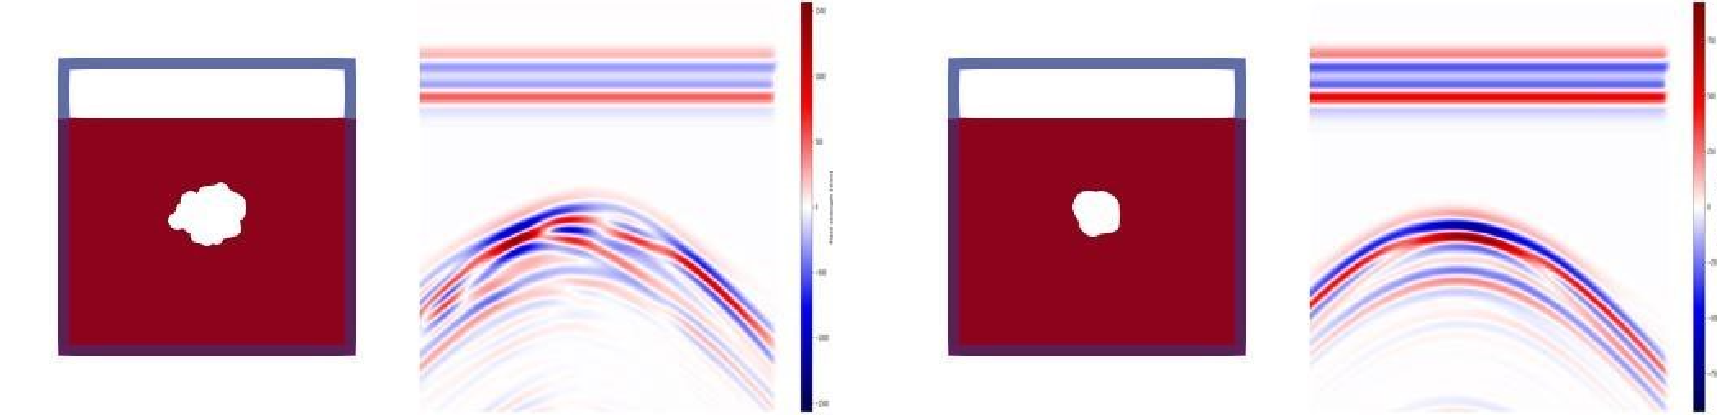
\includegraphics[scale=0.4]{gambar/variasi kompleksitas.png}
  \caption{Data dengan Objek Berbentuk Sederhana (Kanan) dan Data dengan Objek Berbentuk Kompleks (Kiri)}
  \label{fig:kompleksData}
\end{figure}

Pada kategori variasi ukuran objek, data dibedakan berdasar besar ukuran objek, yaitu data dengan objek kecil dan data dengan objek besar. 
Objek kecil memiliki ukuran sekitar 3-4 cm, sedangkan objek besar memiliki ukuran sekitar 5-6 cm. 
Jumlah objek penyusun serta posisi objek disamakan, yaitu objek penyusun sejumlah 5 buah dan kedalaman sekitar 4.5 cm. 
Contoh data untuk variasi ini dapat dilihat pada gambar \ref{fig:ukuranData}.

\begin{figure}[ht]
  \centering
  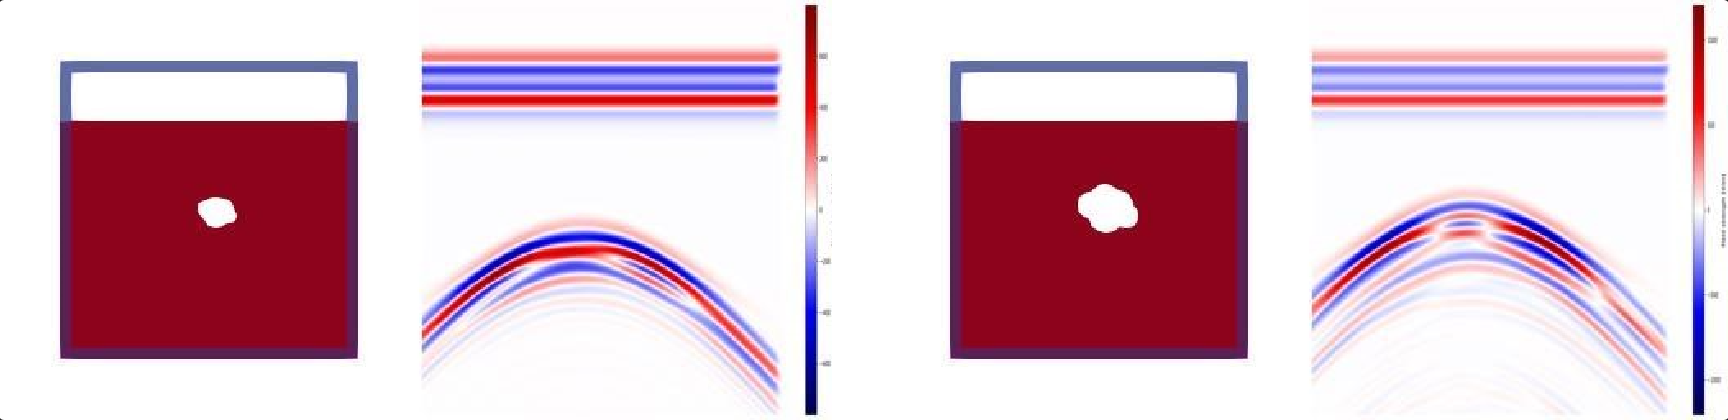
\includegraphics[scale=0.4]{gambar/variasi ukuran.png}
  \caption{Data dengan Objek Berukuran Besar (Kanan) dan Data dengan Objek Berukuran Kecil (Kiri)}
  \label{fig:ukuranData}
\end{figure}

Pada kategori variasi Posisi objek di bawah permukaan, data dibedakan berdasar posisi objek dari permukaan, yaitu data dengan objek dangkal dan data dengan objek dalam. 
Objek dangkal memiliki posisi sekitar 2.5 cm dari permukaan, sedangkan objek dalam memiliki posisi sekitar 7.5 cm dari permukaan. 
Ukuran objek dan jumlah objek penyusun disamakan, yaitu ukuran objek sekitar 4.5 cm dan jumlah objek penyusun sejumlah 5 buah. 
Contoh data untuk variasi ini dapat dilihat pada gambar \ref{fig:posisiData}.

\begin{figure}[ht]
  \centering
  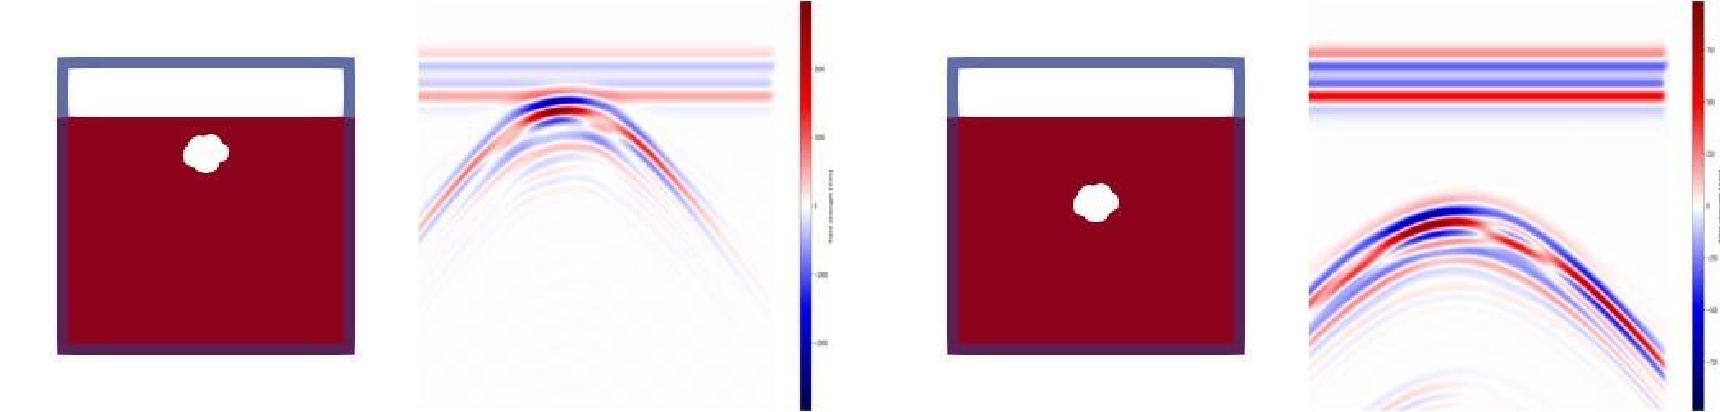
\includegraphics[scale=0.4]{gambar/variasi kedalaman.png}
  \caption{Data dengan Posisi Objek Jauh dari Permukaan (Kanan) dan Data dengan Posisi Objek Dekat dari Permukaan (Kiri)}
  \label{fig:posisiData}
\end{figure}

Pada kategori variasi objek berbentuk regular, data dibedakan berdasar bentuk reguler objek, yaitu data dengan objek berbentuk lingkaran (silinder tampak depan) dan data dengan objek berbentuk segi empat (silinder tampak samping). 
Objek hanya terdiri dari 1 objek penyusun, dengan posisi dan ukuran yang dibebaskan, yaitu posisi sekitar 2.5-10 cm di bawah permukaan dan ukuran sekitar 3-10 cm. 
Contoh data untuk variasi ini dapat dilihat pada gambar \ref{fig:regularData}.

\begin{figure}[ht]
  \centering
  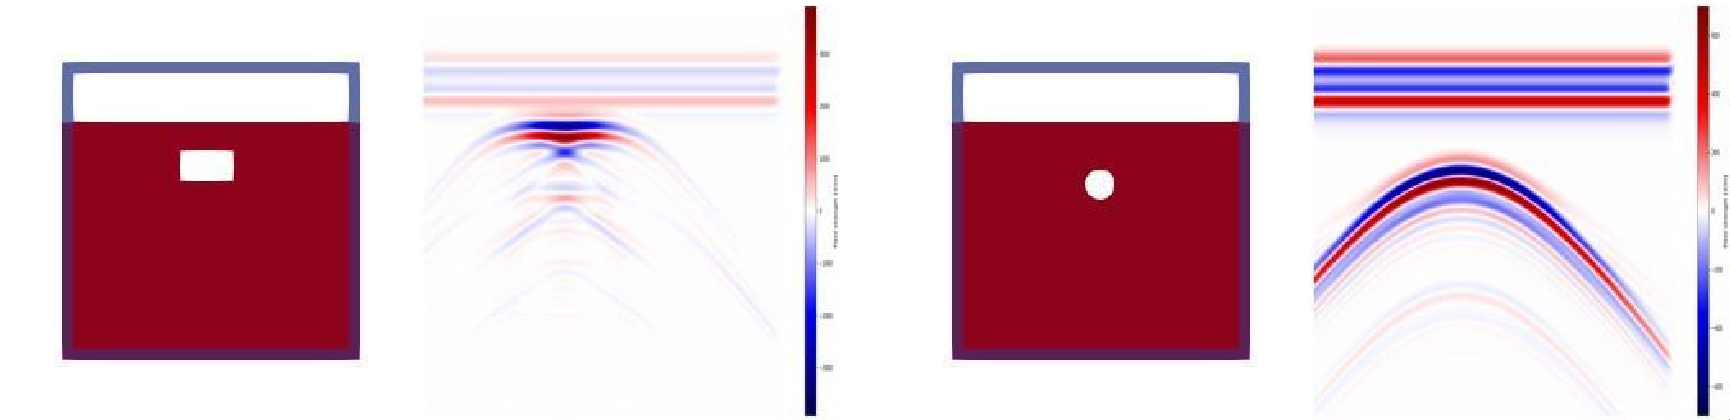
\includegraphics[scale=0.4]{gambar/variasi reguler.png}
  \caption{Data dengan Objek Berbentuk Lingkaran (Kanan) dan Data dengan Objek Berbentuk Segi Empat (Kiri)}
  \label{fig:regularData}
\end{figure}
\newpage

\section{Hasil Pelatihan Model GAN}
\label{sec:hasilpelatihanGAN}

Proses pelatihan model dilakukan sebanyak 40.000 iterasi. 
Total waktu yang diperlukan untuk menjalankan keseluruhan proses pelatihan selama 9 jam mulai jam 20.00 WIB hingga pukul 05.00 WIB esok harinya. 
Selama pelatihan, nilai \emph{total discriminator loss} dan \emph{total generator loss} disimpan ke sebuah \emph{log}. 
Dengan menggunakan tensorboard, nilai \emph{loss} yang disimpan pada \emph{log} dapat divisualisasikan dalam bentuk grafik. 

\begin{figure}[ht]
  \centering
  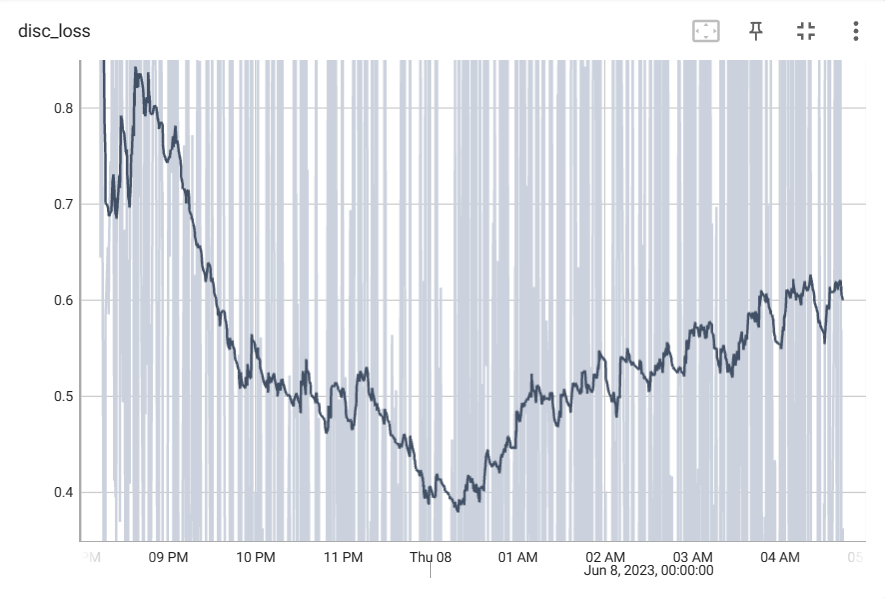
\includegraphics[scale=0.6]{gambar/Disc_loss.png}
  \caption{Grafik Total Discriminator Loss}
  \label{fig:discLoss}
\end{figure}

Gambar \ref{fig:discLoss} menunjukkan grafik \emph{discriminator loss} yang awalnya semakin mengecil kemudian mengalami peningkatan. 
Hal ini menunjukkan bahwa discriminator awalnya semakin baik dalam mempelajari perbedaan data asli dengan data yang disintesis. 
Setelah melewati waktu tertentu, discriminator kemudian menjadi semakin sulit dalam mempelajari perbedaan tersebut. 

\begin{figure}[ht]
  \centering
  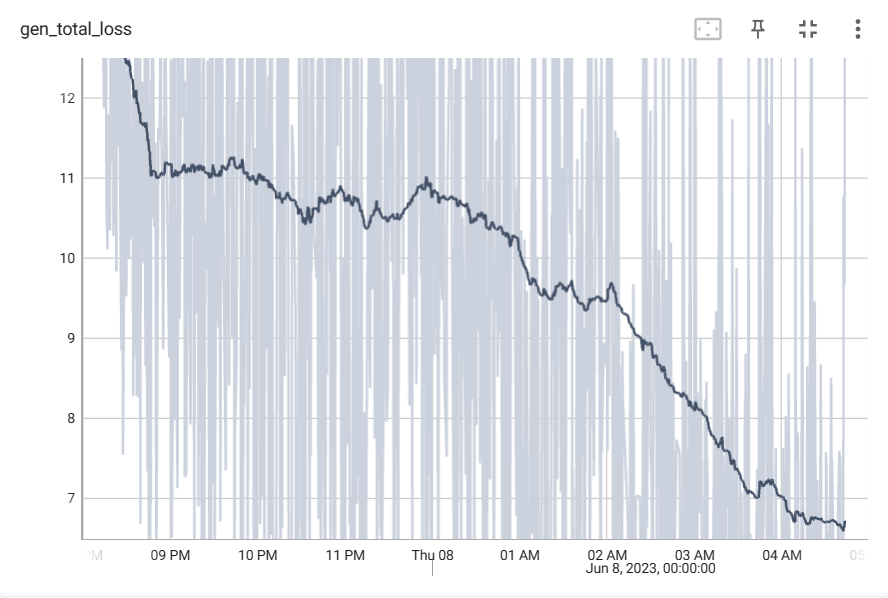
\includegraphics[scale=0.6]{gambar/Gen_total_loss.png}
  \caption{Grafik Total Generator Loss}
  \label{fig:genLoss}
\end{figure}

Gambar \ref{fig:genLoss} menunjukkan grafik \emph{generator loss} yang semakin lama semakin mengecil. 
Hal ini menunjukkan bahwa generator semakin baik dalam mempelajari dan menghasilkan data sintesis yang sesuai dengan data asli. 
Grafik juga menunjukkan penurunan nilai yang lumayan konstan, sehingga dapat dikatakan model generator dilatih secara baik pada proses pelatihan model GAN.

Dalam proses pelatihan model GAN, penting untuk membandingkan nilai atau grafik \emph{generator loss} dan \emph{discriminator loss}. 
Pada kedua grafik, dapat dilihat bahwa awalnya perubahan kedua nilai \emph{loss} sama-sama menurun, yang menunjukkan proses model dalam mempelajari data berjalan dengan baik. 
Namun, sekitar pukul 00.00 grafik dari \emph{discriminator loss} menjadi semakin meningkat, sedangkan grafik \emph{generator loss} tetap semakin menurun. 
Hal ini menunjukkan bahwa pada interval waktu tersebut, discriminator sudah mulai kesulitan dalam membedakan gambar asli dengan gambar palsu, sedangkan generator tetap semakin baik dalam menghasilkan output yang sesuai dengan aslinya.
\newpage
\section{Hasil Evaluasi Output GAN}
\label{sec:evaluasiOutput}

Proses evaluasi dilakukan dengan evaluasi matriks output model kemudian dilanjut dengan evaluasi visual. 
Evaluasi matriks dilakukan dengan menggunakan 3 metode, yaitu metode RMS, MSE, dan SSIM. 
Untuk nilai hasil RMS dan MSE dikatakan baik jika nilainya semakin mendekati 0, sedangkan untuk nilai hasil SSIM dikatakan baik jika nilainya semakin mendekati 1. 
Hasil dari evaluasi matriks untuk keseluruhan data dapat dilihat pada tabel \ref{tb:evaluasimatriks}. 

\begin{table}[]
  \caption{Tabel Nilai RMS, MSE dan SSIM dari Gambar Sintesis dengan Gambar Asli Setiap Variasi Data}
  \label{tb:evaluasimatriks}
  \begin{tabular}{|l|cc|cc|cc|}
  \hline
  \multicolumn{1}{|c|}{Variasi Data}                  & \multicolumn{2}{c|}{RMS}                                                                               & \multicolumn{2}{c|}{MSE}                                                                                   & \multicolumn{2}{c|}{SSIM}                                                                            \\ \hline
                                                      & \multicolumn{1}{c|}{\cellcolor[HTML]{FFFFFF}0.256} & \cellcolor[HTML]{FFFFFF}                         & \multicolumn{1}{c|}{\cellcolor[HTML]{FFFFFF}0.072}  & \cellcolor[HTML]{FFFFFF}                           & \multicolumn{1}{c|}{\cellcolor[HTML]{FFFFFF}0.848} & \cellcolor[HTML]{FFFFFF}                        \\ \cline{2-2} \cline{4-4} \cline{6-6}
                                                      & \multicolumn{1}{c|}{\cellcolor[HTML]{FFFFFF}0.271} & \cellcolor[HTML]{FFFFFF}                         & \multicolumn{1}{c|}{\cellcolor[HTML]{FFFFFF}0.082}  & \cellcolor[HTML]{FFFFFF}                           & \multicolumn{1}{c|}{\cellcolor[HTML]{FFFFFF}0.811} & \cellcolor[HTML]{FFFFFF}                        \\ \cline{2-2} \cline{4-4} \cline{6-6}
                                                      & \multicolumn{1}{c|}{\cellcolor[HTML]{FFFFFF}0.265} & \cellcolor[HTML]{FFFFFF}                         & \multicolumn{1}{c|}{\cellcolor[HTML]{FFFFFF}0.078}  & \cellcolor[HTML]{FFFFFF}                           & \multicolumn{1}{c|}{\cellcolor[HTML]{FFFFFF}0.833} & \cellcolor[HTML]{FFFFFF}                        \\ \cline{2-2} \cline{4-4} \cline{6-6}
                                                      & \multicolumn{1}{c|}{\cellcolor[HTML]{FFFFFF}0.234} & \cellcolor[HTML]{FFFFFF}                         & \multicolumn{1}{c|}{\cellcolor[HTML]{FFFFFF}0.063}  & \cellcolor[HTML]{FFFFFF}                           & \multicolumn{1}{c|}{\cellcolor[HTML]{FFFFFF}0.837} & \cellcolor[HTML]{FFFFFF}                        \\ \cline{2-2} \cline{4-4} \cline{6-6}
  \multirow{-5}{*}{Bentuk Objek Sederhana}          & \multicolumn{1}{c|}{\cellcolor[HTML]{FFFFFF}0.249} & \multirow{-5}{*}{\cellcolor[HTML]{FFFFFF}0.255}  & \multicolumn{1}{c|}{\cellcolor[HTML]{FFFFFF}0.071}  & \multirow{-5}{*}{\cellcolor[HTML]{FFFFFF}0.073}       & \multicolumn{1}{c|}{\cellcolor[HTML]{FFFFFF}0.816} & \multirow{-5}{*}{\cellcolor[HTML]{FFFFFF}0.829} \\ \hline
                                                      & \multicolumn{1}{c|}{0.260}                         & \cellcolor[HTML]{FFFFFF}                         & \multicolumn{1}{c|}{0.075}                         & \cellcolor[HTML]{FFFFFF}                           & \multicolumn{1}{c|}{0.841}                         & \cellcolor[HTML]{FFFFFF}                        \\ \cline{2-2} \cline{4-4} \cline{6-6}
                                                      & \multicolumn{1}{l|}{0.246}                         & \cellcolor[HTML]{FFFFFF}                         & \multicolumn{1}{l|}{0.068}                         & \cellcolor[HTML]{FFFFFF}                           & \multicolumn{1}{l|}{0.830}                         & \cellcolor[HTML]{FFFFFF}                        \\ \cline{2-2} \cline{4-4} \cline{6-6}
                                                      & \multicolumn{1}{l|}{0.266}                         & \cellcolor[HTML]{FFFFFF}                         & \multicolumn{1}{l|}{0.077}                          & \cellcolor[HTML]{FFFFFF}                           & \multicolumn{1}{l|}{0.832}                         & \cellcolor[HTML]{FFFFFF}                        \\ \cline{2-2} \cline{4-4} \cline{6-6}
                                                      & \multicolumn{1}{l|}{0.260}                         & \cellcolor[HTML]{FFFFFF}                         & \multicolumn{1}{l|}{0.074}                         & \cellcolor[HTML]{FFFFFF}                           & \multicolumn{1}{l|}{0.837}                         & \cellcolor[HTML]{FFFFFF}                        \\ \cline{2-2} \cline{4-4} \cline{6-6}
  \multirow{-5}{*}{Bentuk Objek Kompleks}         & \multicolumn{1}{l|}{0.264}                         & \multirow{-5}{*}{\cellcolor[HTML]{FFFFFF}0.259} & \multicolumn{1}{l|}{0.080}                         & \multirow{-5}{*}{\cellcolor[HTML]{FFFFFF}0.075} & \multicolumn{1}{l|}{0.821}                         & \multirow{-5}{*}{\cellcolor[HTML]{FFFFFF}0.832} \\ \hline
                                                      & \multicolumn{1}{c|}{\cellcolor[HTML]{FFFFFF}0.283} & \cellcolor[HTML]{FFFFFF}                         & \multicolumn{1}{c|}{\cellcolor[HTML]{FFFFFF}0.091} & \cellcolor[HTML]{FFFFFF}                           & \multicolumn{1}{c|}{\cellcolor[HTML]{FFFFFF}0.799} & \cellcolor[HTML]{FFFFFF}                        \\ \cline{2-2} \cline{4-4} \cline{6-6}
                                                      & \multicolumn{1}{c|}{\cellcolor[HTML]{FFFFFF}0.256} & \cellcolor[HTML]{FFFFFF}                         & \multicolumn{1}{c|}{\cellcolor[HTML]{FFFFFF}0.073} & \cellcolor[HTML]{FFFFFF}                           & \multicolumn{1}{c|}{\cellcolor[HTML]{FFFFFF}0.831} & \cellcolor[HTML]{FFFFFF}                        \\ \cline{2-2} \cline{4-4} \cline{6-6}
                                                      & \multicolumn{1}{c|}{\cellcolor[HTML]{FFFFFF}0.231} & \cellcolor[HTML]{FFFFFF}                         & \multicolumn{1}{c|}{\cellcolor[HTML]{FFFFFF}0.065} & \cellcolor[HTML]{FFFFFF}                           & \multicolumn{1}{c|}{\cellcolor[HTML]{FFFFFF}0.829} & \cellcolor[HTML]{FFFFFF}                        \\ \cline{2-2} \cline{4-4} \cline{6-6}
                                                      & \multicolumn{1}{c|}{\cellcolor[HTML]{FFFFFF}0.246} & \cellcolor[HTML]{FFFFFF}                         & \multicolumn{1}{c|}{\cellcolor[HTML]{FFFFFF}0.066} & \cellcolor[HTML]{FFFFFF}                           & \multicolumn{1}{c|}{\cellcolor[HTML]{FFFFFF}0.857} & \cellcolor[HTML]{FFFFFF}                        \\ \cline{2-2} \cline{4-4} \cline{6-6}
  \multirow{-5}{*}{Ukuran Objek Kecil}            & \multicolumn{1}{c|}{\cellcolor[HTML]{FFFFFF}0.251} & \multirow{-5}{*}{\cellcolor[HTML]{FFFFFF}0.254} & \multicolumn{1}{c|}{\cellcolor[HTML]{FFFFFF}0.069} & \multirow{-5}{*}{\cellcolor[HTML]{FFFFFF}0.073} & \multicolumn{1}{c|}{\cellcolor[HTML]{FFFFFF}0.829} & \multirow{-5}{*}{\cellcolor[HTML]{FFFFFF}0.829} \\ \hline
                                                      & \multicolumn{1}{c|}{\cellcolor[HTML]{FFFFFF}0.267} & \cellcolor[HTML]{FFFFFF}                         & \multicolumn{1}{c|}{\cellcolor[HTML]{FFFFFF}0.081} & \cellcolor[HTML]{FFFFFF}                           & \multicolumn{1}{c|}{\cellcolor[HTML]{FFFFFF}0.818} & \cellcolor[HTML]{FFFFFF}                        \\ \cline{2-2} \cline{4-4} \cline{6-6}
                                                      & \multicolumn{1}{c|}{\cellcolor[HTML]{FFFFFF}0.259} & \cellcolor[HTML]{FFFFFF}                         & \multicolumn{1}{c|}{\cellcolor[HTML]{FFFFFF}0.076} & \cellcolor[HTML]{FFFFFF}                           & \multicolumn{1}{c|}{\cellcolor[HTML]{FFFFFF}0.817} & \cellcolor[HTML]{FFFFFF}                        \\ \cline{2-2} \cline{4-4} \cline{6-6}
                                                      & \multicolumn{1}{c|}{\cellcolor[HTML]{FFFFFF}0.236} & \cellcolor[HTML]{FFFFFF}                         & \multicolumn{1}{c|}{\cellcolor[HTML]{FFFFFF}0.068} & \cellcolor[HTML]{FFFFFF}                           & \multicolumn{1}{c|}{\cellcolor[HTML]{FFFFFF}0.825} & \cellcolor[HTML]{FFFFFF}                        \\ \cline{2-2} \cline{4-4} \cline{6-6}
                                                      & \multicolumn{1}{c|}{\cellcolor[HTML]{FFFFFF}0.279} & \cellcolor[HTML]{FFFFFF}                         & \multicolumn{1}{c|}{\cellcolor[HTML]{FFFFFF}0.084} & \cellcolor[HTML]{FFFFFF}                           & \multicolumn{1}{c|}{\cellcolor[HTML]{FFFFFF}0.833} & \cellcolor[HTML]{FFFFFF}                        \\ \cline{2-2} \cline{4-4} \cline{6-6}
  \multirow{-5}{*}{Ukuran Objek Besar}             & \multicolumn{1}{c|}{\cellcolor[HTML]{FFFFFF}0.275} & \multirow{-5}{*}{\cellcolor[HTML]{FFFFFF}0.263} & \multicolumn{1}{c|}{\cellcolor[HTML]{FFFFFF}0.083} & \multirow{-5}{*}{\cellcolor[HTML]{FFFFFF}0.078} & \multicolumn{1}{c|}{\cellcolor[HTML]{FFFFFF}0.826} & \multirow{-5}{*}{\cellcolor[HTML]{FFFFFF}0.824} \\ \hline
                                                      & \multicolumn{1}{c|}{\cellcolor[HTML]{FFFFFF}0.241} & \cellcolor[HTML]{FFFFFF}                         & \multicolumn{1}{c|}{\cellcolor[HTML]{FFFFFF}0.061} & \cellcolor[HTML]{FFFFFF}                           & \multicolumn{1}{c|}{\cellcolor[HTML]{FFFFFF}0.842} & \cellcolor[HTML]{FFFFFF}                        \\ \cline{2-2} \cline{4-4} \cline{6-6}
                                                      & \multicolumn{1}{c|}{\cellcolor[HTML]{FFFFFF}0.231} & \cellcolor[HTML]{FFFFFF}                         & \multicolumn{1}{c|}{\cellcolor[HTML]{FFFFFF}0.060}  & \cellcolor[HTML]{FFFFFF}                           & \multicolumn{1}{c|}{\cellcolor[HTML]{FFFFFF}0.847} & \cellcolor[HTML]{FFFFFF}                        \\ \cline{2-2} \cline{4-4} \cline{6-6}
                                                      & \multicolumn{1}{c|}{\cellcolor[HTML]{FFFFFF}0.246} & \cellcolor[HTML]{FFFFFF}                         & \multicolumn{1}{c|}{\cellcolor[HTML]{FFFFFF}0.069} & \cellcolor[HTML]{FFFFFF}                           & \multicolumn{1}{c|}{\cellcolor[HTML]{FFFFFF}0.821} & \cellcolor[HTML]{FFFFFF}                        \\ \cline{2-2} \cline{4-4} \cline{6-6}
                                                      & \multicolumn{1}{c|}{\cellcolor[HTML]{FFFFFF}0.224} & \cellcolor[HTML]{FFFFFF}                         & \multicolumn{1}{c|}{\cellcolor[HTML]{FFFFFF}0.057}  & \cellcolor[HTML]{FFFFFF}                           & \multicolumn{1}{c|}{\cellcolor[HTML]{FFFFFF}0.847} & \cellcolor[HTML]{FFFFFF}                        \\ \cline{2-2} \cline{4-4} \cline{6-6}
  \multirow{-5}{*}{Posisi Objek Dekat dari Permukaan}                & \multicolumn{1}{c|}{\cellcolor[HTML]{FFFFFF}0.252} & \multirow{-5}{*}{\cellcolor[HTML]{FFFFFF}0.239} & \multicolumn{1}{c|}{\cellcolor[HTML]{FFFFFF}0.070} & \multirow{-5}{*}{\cellcolor[HTML]{FFFFFF}0.063} & \multicolumn{1}{c|}{\cellcolor[HTML]{FFFFFF}0.846} & \multirow{-5}{*}{\cellcolor[HTML]{FFFFFF}0.841} \\ \hline
                                                      & \multicolumn{1}{c|}{\cellcolor[HTML]{FFFFFF}0.257} & \cellcolor[HTML]{FFFFFF}                         & \multicolumn{1}{c|}{\cellcolor[HTML]{FFFFFF}0.076} & \cellcolor[HTML]{FFFFFF}                           & \multicolumn{1}{c|}{\cellcolor[HTML]{FFFFFF}0.812} & \cellcolor[HTML]{FFFFFF}                        \\ \cline{2-2} \cline{4-4} \cline{6-6}
                                                      & \multicolumn{1}{c|}{\cellcolor[HTML]{FFFFFF}0.255} & \cellcolor[HTML]{FFFFFF}                         & \multicolumn{1}{c|}{\cellcolor[HTML]{FFFFFF}0.073} & \cellcolor[HTML]{FFFFFF}                           & \multicolumn{1}{c|}{\cellcolor[HTML]{FFFFFF}0.828} & \cellcolor[HTML]{FFFFFF}                        \\ \cline{2-2} \cline{4-4} \cline{6-6}
                                                      & \multicolumn{1}{c|}{\cellcolor[HTML]{FFFFFF}0.252} & \cellcolor[HTML]{FFFFFF}                         & \multicolumn{1}{c|}{\cellcolor[HTML]{FFFFFF}0.069} & \cellcolor[HTML]{FFFFFF}                           & \multicolumn{1}{c|}{\cellcolor[HTML]{FFFFFF}0.851} & \cellcolor[HTML]{FFFFFF}                        \\ \cline{2-2} \cline{4-4} \cline{6-6}
                                                      & \multicolumn{1}{c|}{\cellcolor[HTML]{FFFFFF}0.263} & \cellcolor[HTML]{FFFFFF}                         & \multicolumn{1}{c|}{\cellcolor[HTML]{FFFFFF}0.075} & \cellcolor[HTML]{FFFFFF}                           & \multicolumn{1}{c|}{\cellcolor[HTML]{FFFFFF}0.823} & \cellcolor[HTML]{FFFFFF}                        \\ \cline{2-2} \cline{4-4} \cline{6-6}
  \multirow{-5}{*}{Posisi Objek Jauh dari Permukaan}                & \multicolumn{1}{c|}{\cellcolor[HTML]{FFFFFF}0.231} & \multirow{-5}{*}{\cellcolor[HTML]{FFFFFF}0.252} & \multicolumn{1}{c|}{\cellcolor[HTML]{FFFFFF}0.065} & \multirow{-5}{*}{\cellcolor[HTML]{FFFFFF}0.072} & \multicolumn{1}{c|}{\cellcolor[HTML]{FFFFFF}0.831} & \multirow{-5}{*}{\cellcolor[HTML]{FFFFFF}0.829} \\ \hline
                                                      & \multicolumn{1}{c|}{\cellcolor[HTML]{FFFFFF}0.206} & \cellcolor[HTML]{FFFFFF}                         & \multicolumn{1}{c|}{\cellcolor[HTML]{FFFFFF}0.048} & \cellcolor[HTML]{FFFFFF}                           & \multicolumn{1}{c|}{\cellcolor[HTML]{FFFFFF}0.861} & \cellcolor[HTML]{FFFFFF}                        \\ \cline{2-2} \cline{4-4} \cline{6-6}
                                                      & \multicolumn{1}{c|}{\cellcolor[HTML]{FFFFFF}0.217} & \cellcolor[HTML]{FFFFFF}                         & \multicolumn{1}{c|}{\cellcolor[HTML]{FFFFFF}0.056}  & \cellcolor[HTML]{FFFFFF}                           & \multicolumn{1}{c|}{\cellcolor[HTML]{FFFFFF}0.844} & \cellcolor[HTML]{FFFFFF}                        \\ \cline{2-2} \cline{4-4} \cline{6-6}
                                                      & \multicolumn{1}{c|}{\cellcolor[HTML]{FFFFFF}0.264} & \cellcolor[HTML]{FFFFFF}                         & \multicolumn{1}{c|}{\cellcolor[HTML]{FFFFFF}0.078} & \cellcolor[HTML]{FFFFFF}                           & \multicolumn{1}{c|}{\cellcolor[HTML]{FFFFFF}0.826} & \cellcolor[HTML]{FFFFFF}                        \\ \cline{2-2} \cline{4-4} \cline{6-6}
                                                      & \multicolumn{1}{c|}{\cellcolor[HTML]{FFFFFF}0.252} & \cellcolor[HTML]{FFFFFF}                         & \multicolumn{1}{c|}{\cellcolor[HTML]{FFFFFF}0.071} & \cellcolor[HTML]{FFFFFF}                           & \multicolumn{1}{c|}{\cellcolor[HTML]{FFFFFF}0.841} & \cellcolor[HTML]{FFFFFF}                        \\ \cline{2-2} \cline{4-4} \cline{6-6}
  \multirow{-5}{*}{Bentuk Objek Lingkaran} & \multicolumn{1}{c|}{\cellcolor[HTML]{FFFFFF}0.249} & \multirow{-5}{*}{\cellcolor[HTML]{FFFFFF}0.237} & \multicolumn{1}{c|}{\cellcolor[HTML]{FFFFFF}0.069} & \multirow{-5}{*}{\cellcolor[HTML]{FFFFFF}0.064} & \multicolumn{1}{c|}{\cellcolor[HTML]{FFFFFF}0.843} & \multirow{-5}{*}{\cellcolor[HTML]{FFFFFF}0.843} \\ \hline
                                                      & \multicolumn{1}{c|}{\cellcolor[HTML]{FFFFFF}0.205} & \cellcolor[HTML]{FFFFFF}                         & \multicolumn{1}{c|}{\cellcolor[HTML]{FFFFFF}0.053} & \cellcolor[HTML]{FFFFFF}                           & \multicolumn{1}{c|}{\cellcolor[HTML]{FFFFFF}0.843} & \cellcolor[HTML]{FFFFFF}                        \\ \cline{2-2} \cline{4-4} \cline{6-6}
                                                      & \multicolumn{1}{c|}{\cellcolor[HTML]{FFFFFF}0.197} & \cellcolor[HTML]{FFFFFF}                         & \multicolumn{1}{c|}{\cellcolor[HTML]{FFFFFF}0.047} & \cellcolor[HTML]{FFFFFF}                           & \multicolumn{1}{c|}{\cellcolor[HTML]{FFFFFF}0.849} & \cellcolor[HTML]{FFFFFF}                        \\ \cline{2-2} \cline{4-4} \cline{6-6}
                                                      & \multicolumn{1}{c|}{\cellcolor[HTML]{FFFFFF}0.204} & \cellcolor[HTML]{FFFFFF}                         & \multicolumn{1}{c|}{\cellcolor[HTML]{FFFFFF}0.049}  & \cellcolor[HTML]{FFFFFF}                           & \multicolumn{1}{c|}{\cellcolor[HTML]{FFFFFF}0.857} & \cellcolor[HTML]{FFFFFF}                        \\ \cline{2-2} \cline{4-4} \cline{6-6}
                                                      & \multicolumn{1}{c|}{\cellcolor[HTML]{FFFFFF}0.257} & \cellcolor[HTML]{FFFFFF}                         & \multicolumn{1}{c|}{\cellcolor[HTML]{FFFFFF}0.075} & \cellcolor[HTML]{FFFFFF}                           & \multicolumn{1}{c|}{\cellcolor[HTML]{FFFFFF}0.833} & \cellcolor[HTML]{FFFFFF}                        \\ \cline{2-2} \cline{4-4} \cline{6-6}
  \multirow{-5}{*}{Bentuk Objek Segi Empat}  & \multicolumn{1}{c|}{\cellcolor[HTML]{FFFFFF}0.233} & \multirow{-5}{*}{\cellcolor[HTML]{FFFFFF}0.219} & \multicolumn{1}{c|}{\cellcolor[HTML]{FFFFFF}0.065} & \multirow{-5}{*}{\cellcolor[HTML]{FFFFFF}0.058} & \multicolumn{1}{c|}{\cellcolor[HTML]{FFFFFF}0.809} & \multirow{-5}{*}{\cellcolor[HTML]{FFFFFF}0.838} \\ \hline
  Rata-Rata                                           & \multicolumn{2}{c|}{\cellcolor[HTML]{FFFFFF}0.247}                                                    & \multicolumn{2}{c|}{0.070}                                                                              & \multicolumn{2}{c|}{0.833}                                                                           \\ \hline
  \end{tabular}
\end{table}

Berdasarkan keseluruhan hasil evaluasi matriks, diperoleh rata-rata RMS = 0.247, MSE = 0.070, dan SSIM = 0.833. 
Ketika pelaksanaan penelitian ini, belum ditemukan standar nilai RMS, MSE, dan SSIM yang bersifat universal atau mutlak untuk menentukan apakah kesamaan 2 buah gambar dianggap cukup identik atau belum. 
Oleh karena itu, nilai rata-rata ini digunakan sebagai standar kemampuan model dalam menghasilkan data untuk setiap variasinya.

Untuk variasi yang nilai rata-rata RMS dan MSE-nya lebih kecil dari nilai rata-rata RMS dan MSE total, dapat dikatakan perbedaan intensitas piksel antara gambar yang disintesis dengan gambar asli cukup dekat. 
Variasi tersebut diantaranya variasi posisi objek dekat dari permukaan, bentuk regular lingkaran, dan bentuk regular segi empat. 
Sebaliknya, untuk variasi yang nilai rata-rata RMS dan MSE-nya lebih besar dari nilai rata-rata RMS dan MSE total, dapat dikatakan perbedaan intensitas piksel antara gambar yang disintesis dengan gambar asli cukup jauh. 
Variasi tersebut diantaranya variasi bentuk objek sederhana, bentuk objek kompleks, ukuran objek kecil, ukuran objek besar, dan posisi objek jauh dari permukaan.

Untuk variasi yang nilai rata-rata SSIM-nya lebih besar dari nilai rata-rata SSIM total, dapat dikatakan kesamaan struktural antara gambar yang disintesis dengan gambar asli hampir sama. 
Variasi tersebut diantaranya variasi posisi objek dekat dari permukaan, bentuk regular lingkaran, dan bentuk regular segi empat. 
Sebaliknya, untuk variasi yang nilai rata-rata SSIM-nya lebih kecil dari nilai rata-rata SSIM total, dapat dikatakan kesamaan struktural antara gambar yang disintesis dengan gambar asli cukup jauh. 
Variasi tersebut diantaranya variasi bentuk objek sederhana, bentuk objek kompleks, ukuran objek kecil, ukuran objek besar, dan posisi objek jauh dari permukaan.

Setelah melakukan evaluasi matriks, dilakukan evaluasi visual. 
Evaluasi visual dilakukan dengan menggunakan fungsi \emph{image differencing}, yang mengurangkan piksel-piksel dari gambar asli dengan gambar sintesis. 
Hasil evaluasi visual akan ditampilkan dengan gambar, dimana semakin gelap (hitam) warna suatu daerah gambar tertentu, maka semakin identik gambar asli dengan gambar sintesis. 
Sebaliknya, semakin terang (putih) warna suatu daerah gambar tertentu, maka semakin berbeda gambar asli dengan gambar sintesis.

Pada variasi kompleksitas bentuk objek, terlihat untuk objek berbentuk sederhana memiliki rata-rata nilai evaluasi matriks yang lebih baik dari objek berbentuk kompleks. 
Perbedaan rata-rata evaluasi matriks terlihat cukup dekat di antara kedua variasi data.  
Nilai rata-rata RMS dan MSE data objek sederhana lebih kecil dari nilai rata-rata RMS dan MSE data objek kompleks. 
Namun, nilai rata-rata SSIM data objek sederhana lebih kecil dari nilai rata-rata SSIM data objek kompleks. 

\begin{figure}[ht]
  \centering
  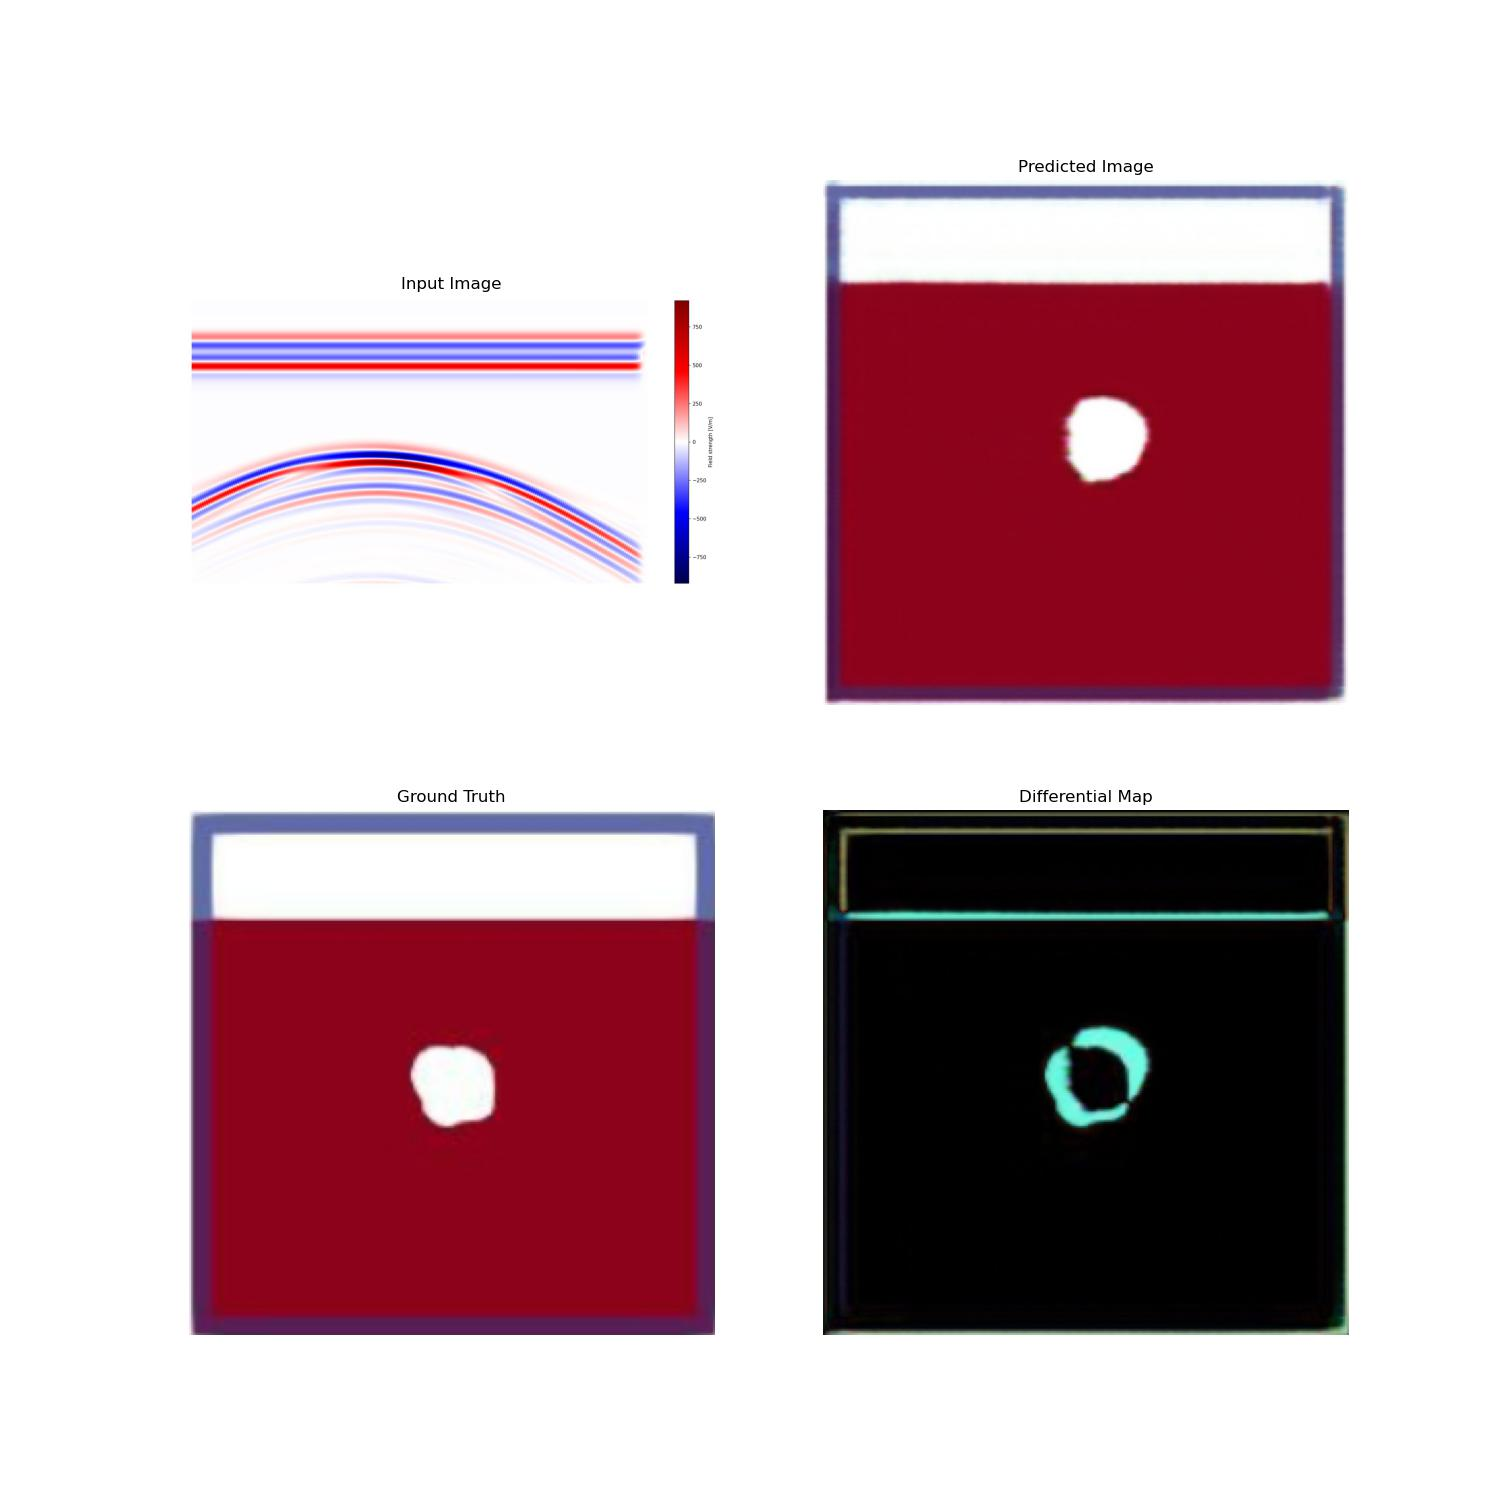
\includegraphics[scale=0.15]{gambar/diffMapSederhana.jpg}
  \caption{Evaluasi Visual Data Variasi Bentuk Sederhana}
  \label{fig:diffmapsederhana}
\end{figure}

Untuk variasi data dengan objek sederhana akan diambil data pertama karena memiliki nilai evaluasi matriks yang lebih mendekati rata-rata variasi bentuk objek dari data lain. 
Evaluasi visual dari data dapat dilihat dari gambar \ref{fig:diffmapsederhana}.
Pada gambar evaluasi visual dapat dilihat bahwa irisan dari objek sintesis dengan objek asli cukup luas sehingga memiliki area error yang cukup sempit. 
Hal ini menunjukkan bahwa output model sudah bisa menunjukkan posisi dan ukuran objek, namun masih belum bisa menunjukkan bentuk objek.

\begin{figure}[ht]
  \centering
  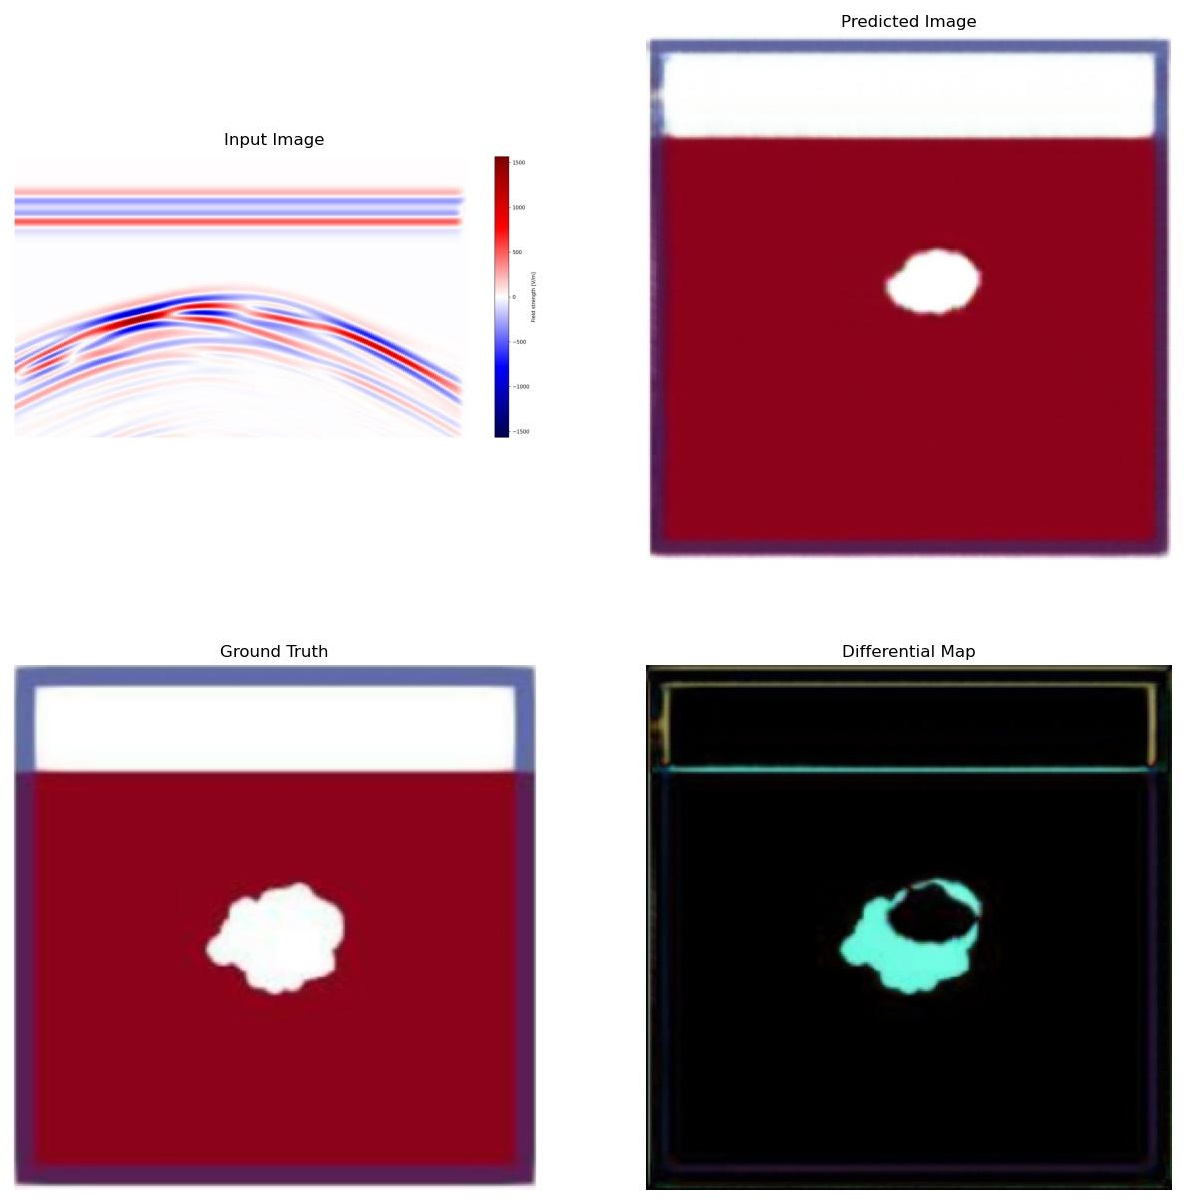
\includegraphics[scale=0.15]{gambar/diffMapKompleks.jpg}
  \caption{Evaluasi Visual Data Variasi Bentuk Kompleks}
  \label{fig:diffmapkompleks}
\end{figure}
\newpage
Untuk variasi data dengan objek kompleks akan diambil data pertama karena memiliki nilai evaluasi matriks yang lebih mendekati rata-rata variasi bentuk objek dari data lain. 
Evaluasi visual dari data dapat dilihat dari gambar \ref{fig:diffmapkompleks}. 
Pada gambar evaluasi visual dapat dilihat bahwa irisan dari gambar sintesis dengan gambar asli hampir merupakan gambar sintesis sepenuhnya. 
Hal ini menunjukkan bahwa output model sudah bisa menunjukkan posisi objek, namun masih belum bisa menunjukkan bentuk dan ukuran objek.

Pada variasi ukuran objek, terlihat untuk objek berukuran kecil memiliki rata-rata nilai evaluasi matriks yang lebih baik dari objek berukuran besar. 
Perbedaan rata-rata evaluasi matriks terlihat cukup jauh di antara kedua variasi data. 
Nilai rata-rata RMS dan MSE data objek berukuran kecil lebih kecil dari nilai rata-rata RMS dan MSE data objek berukuran besar. 
Namun, nilai rata-rata SSIM data objek berukuran kecil lebih besar dari nilai rata-rata SSIM data objek berukuran besar. 

\begin{figure}[ht]
  \centering
  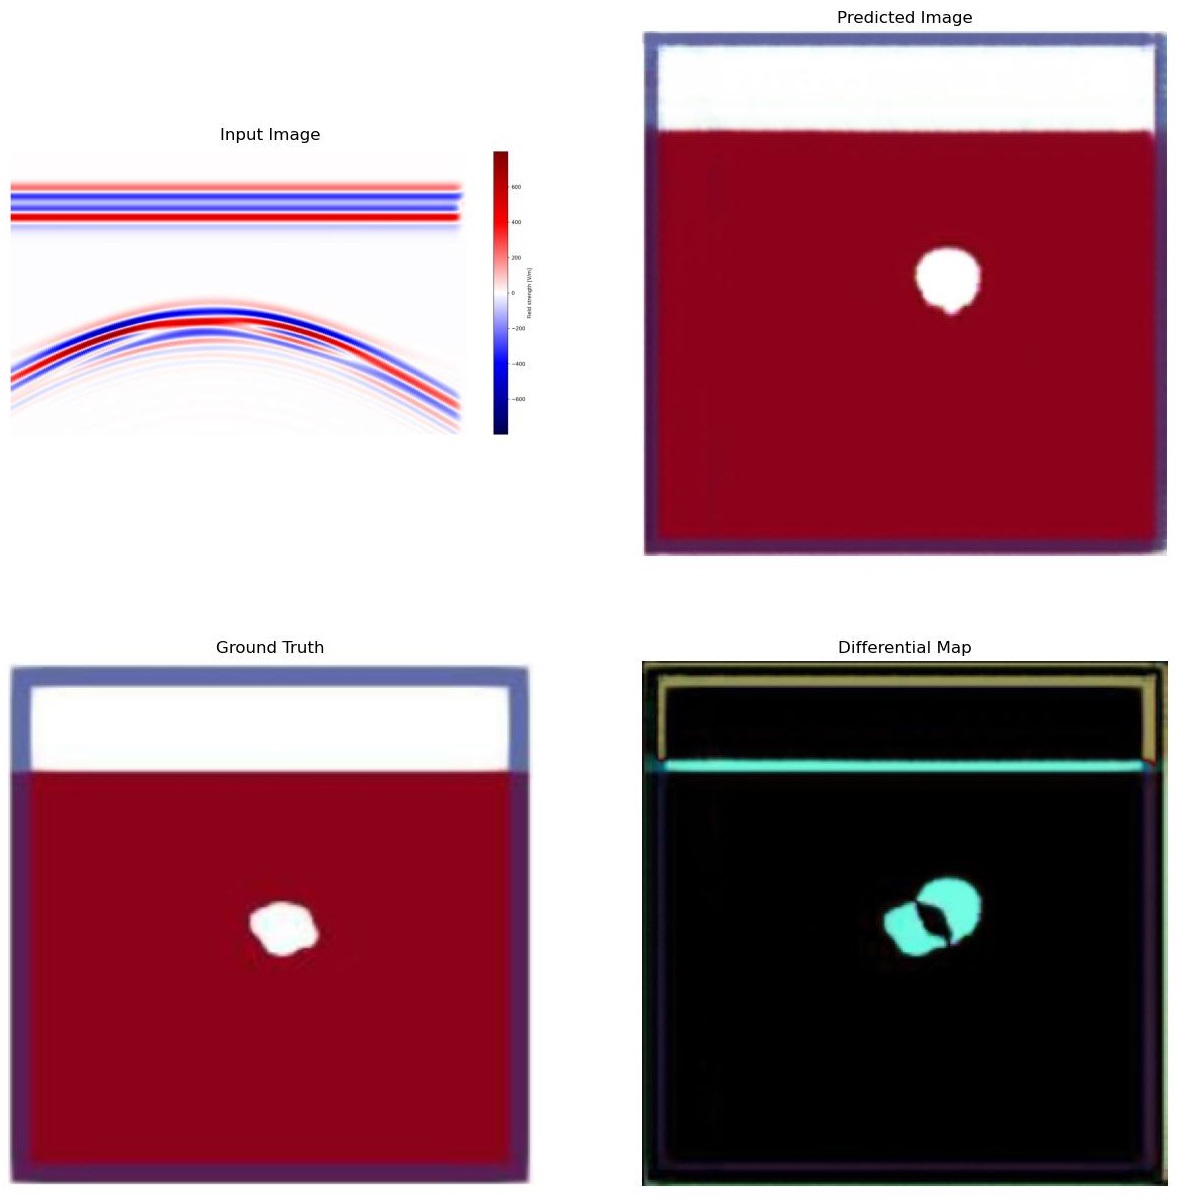
\includegraphics[scale=0.15]{gambar/diffMapKecil.jpg}
  \caption{Evaluasi Visual Data Variasi Ukuran Kecil}
  \label{fig:diffmapkecil}
\end{figure}

Untuk variasi data dengan objek berukuran kecil akan diambil data kelima karena memiliki nilai evaluasi matriks yang lebih mendekati rata-rata variasi ukuran objek dari data lain. 
Evaluasi visual dari data dapat dilihat dari gambar \ref{fig:diffmapkecil}. 
Pada gambar evaluasi visual dapat dilihat bahwa irisan dari objek sintesis dengan objek asli cukup sedikit sehingga memiliki area error yang cukup luas. 
Hal ini menunjukkan bahwa output model hampir bisa menunjukkan posisi dan ukuran objek, namun masih belum bisa menunjukkan bentuk objek.

\begin{figure}[ht]
  \centering
  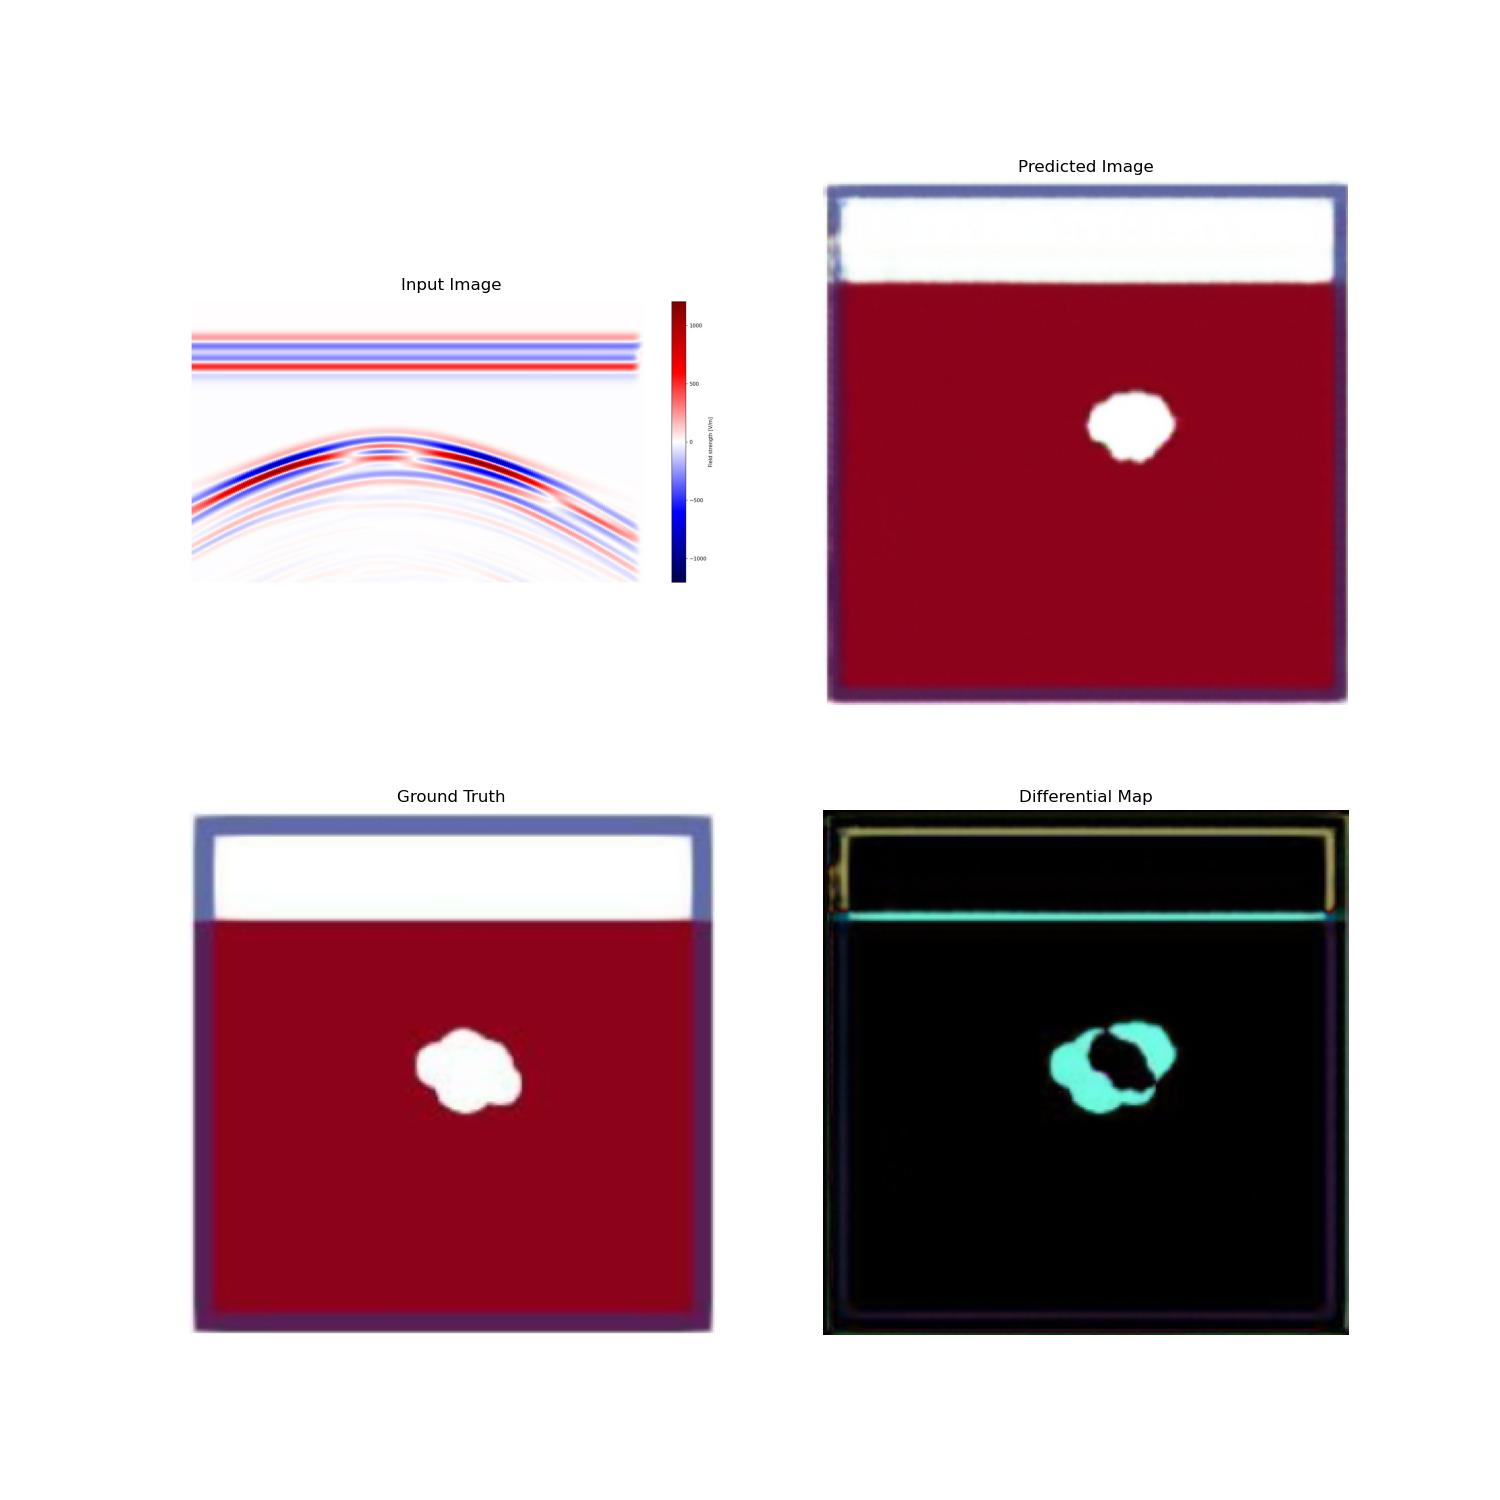
\includegraphics[scale=0.15]{gambar/diffMapBesar.jpg}
  \caption{Evaluasi Visual Data Variasi Ukuran Besar}
  \label{fig:diffmapbesar}
\end{figure}

Untuk variasi data dengan objek berukuran besar akan diambil data pertama karena memiliki nilai evaluasi matriks yang lebih mendekati rata-rata variasi ukuran objek dari data lain. 
Evaluasi visual dari data dapat dilihat dari gambar \ref{fig:diffmapbesar}. 
Pada gambar evaluasi visual dapat dilihat bahwa irisan dari objek sintesis dengan objek asli cukup sempit sehingga memiliki area error yang cukup luas. 
Hal ini menunjukkan bahwa output model hampir bisa menunjukkan posisi objek, namun masih belum bisa menunjukkan bentuk dan ukuran objek.

Pada variasi posisi objek, terlihat untuk objek dengan posisi dekat dengan permukaan memiliki rata-rata nilai evaluasi matriks yang lebih baik dari objek dengan posisi jauh dengan permukaan.
Perbedaan rata-rata evaluasi matriks terlihat cukup jauh di antara kedua variasi data. 
Nilai rata-rata RMS dan MSE data posisi objek dekat dari permukaan lebih kecil dari nilai rata-rata RMS dan MSE data posisi objek jauh dari permukaan. 
Namun, nilai rata-rata SSIM data posisi objek dekat dari permukaan lebih besar dari nilai rata-rata SSIM data posisi objek jauh dari permukaan. 

\begin{figure}[ht]
  \centering
  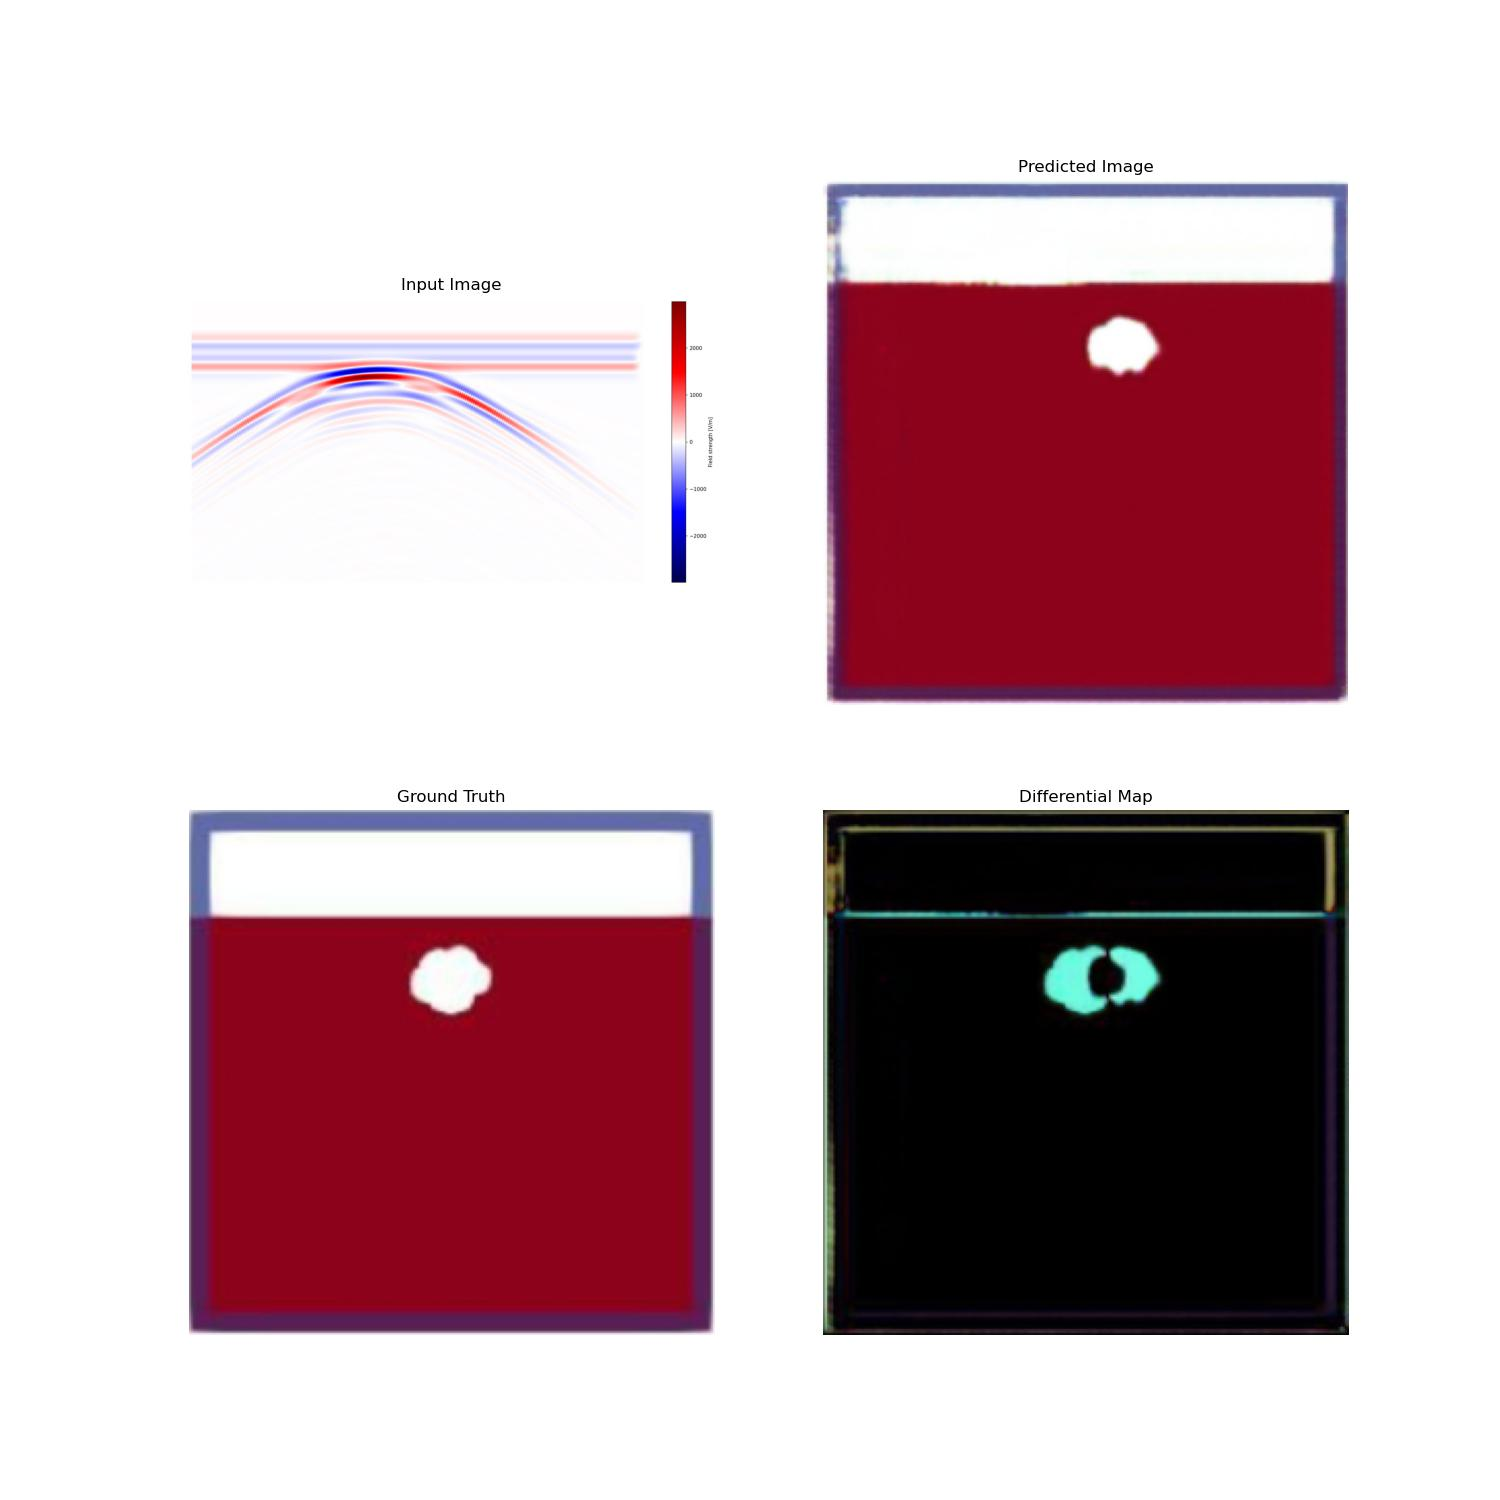
\includegraphics[scale=0.15]{gambar/diffMapDangkal.jpg}
  \caption{Evaluasi Visual Data Variasi Posisi Dekat dengan Permukaan}
  \label{fig:diffmapdangkal}
\end{figure}

Untuk variasi data dengan posisi objek dekat dari permukaan akan diambil data pertama karena memiliki nilai evaluasi matriks yang lebih mendekati rata-rata variasi posisi objek dari data lain. 
Evaluasi visual dari data dapat dilihat dari gambar \ref{fig:diffmapdangkal}. 
Pada gambar evaluasi visual dapat dilihat bahwa irisan dari objek sintesis dengan objek asli cukup sedikit sehingga memiliki area error yang cukup luas. 
Hal ini menunjukkan bahwa output model hampir bisa menunjukkan posisi objek, namun masih belum bisa menunjukkan bentuk dan ukuran objek.

\begin{figure}[ht]
  \centering
  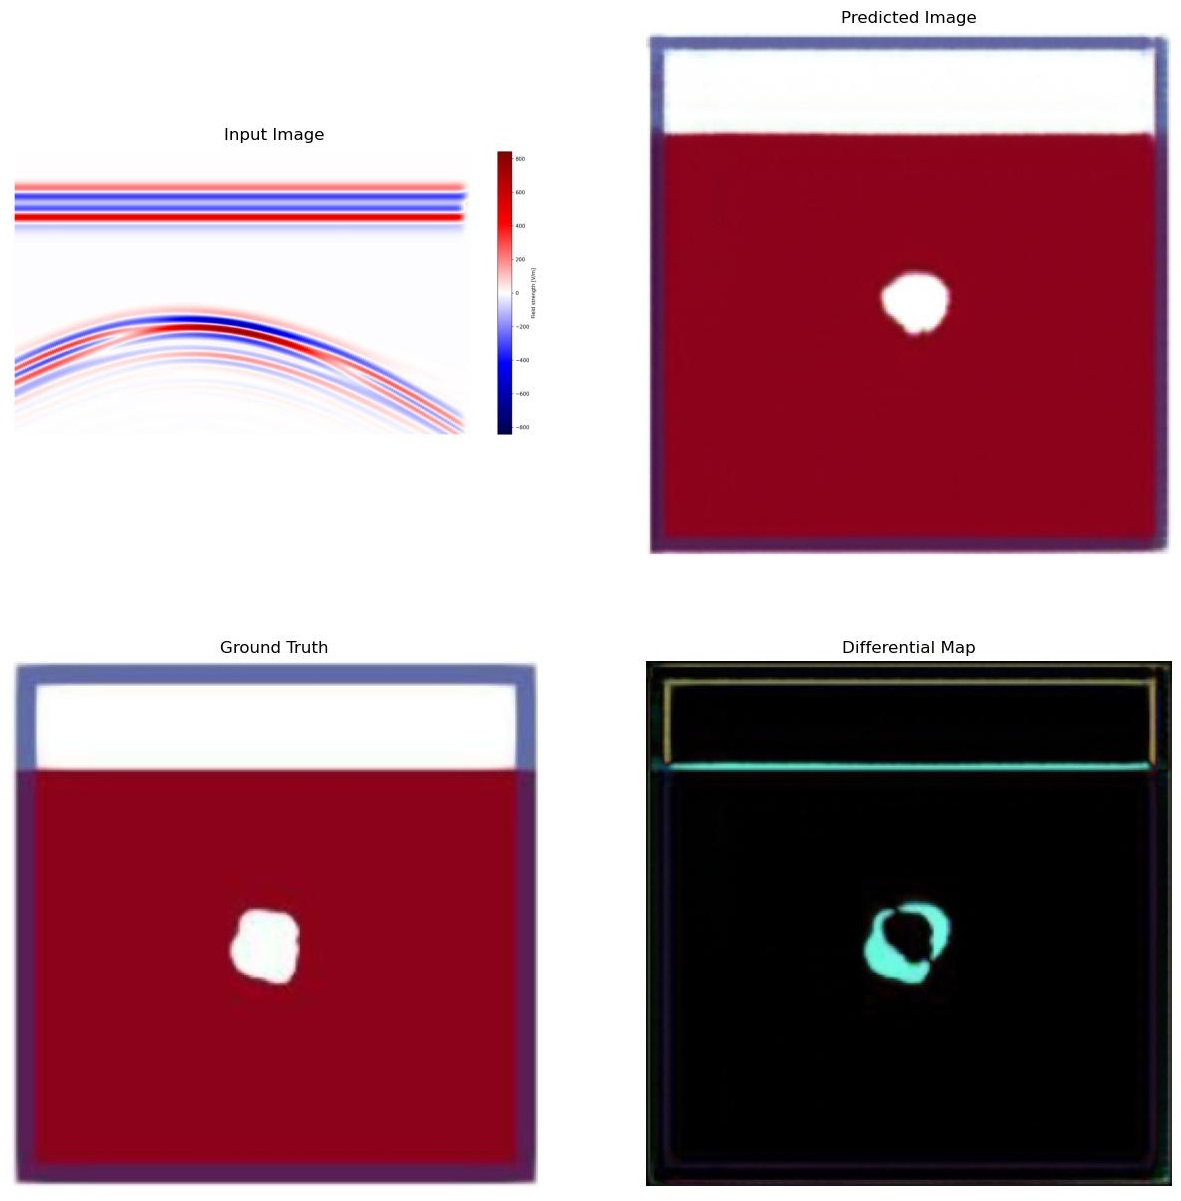
\includegraphics[scale=0.15]{gambar/diffMapDalam.jpg}
  \caption{Evaluasi Visual Data Variasi Posisi Jauh dengan Permukaan}
  \label{fig:diffmapdalam}
\end{figure}
\newpage
Untuk variasi data dengan posisi objek jauh dari permukaan akan diambil data kedua karena memiliki nilai evaluasi matriks yang lebih mendekati rata-rata variasi posisi objek dari data lain. 
Evaluasi visual dari data dapat dilihat dari gambar \ref{fig:diffmapdalam}. 
Pada gambar evaluasi visual dapat dilihat bahwa irisan dari objek sintesis dengan objek asli cukup sedikit sehingga memiliki area error yang cukup luas. 
Hal ini menunjukkan bahwa output model hampir bisa menunjukkan posisi objek, namun masih belum bisa menunjukkan bentuk dan ukuran objek.

Pada variasi bentuk regular objek, terlihat untuk objek berbentuk lingkaran memiliki rata-rata nilai evaluasi matriks yang lebih buruk dari objek berbentuk segi empat.
Perbedaan rata-rata evaluasi matriks terlihat cukup jauh di antara kedua variasi data. 
Nilai rata-rata RMS dan MSE data objek berbentuk lingkaran lebih besar dari nilai rata-rata RMS dan MSE data objek berbentuk segi empat. 
Namun, nilai rata-rata SSIM data objek berbentuk lingkaran lebih besar dari nilai rata-rata SSIM data objek berbentuk segi empat. 

\begin{figure}[ht]
  \centering
  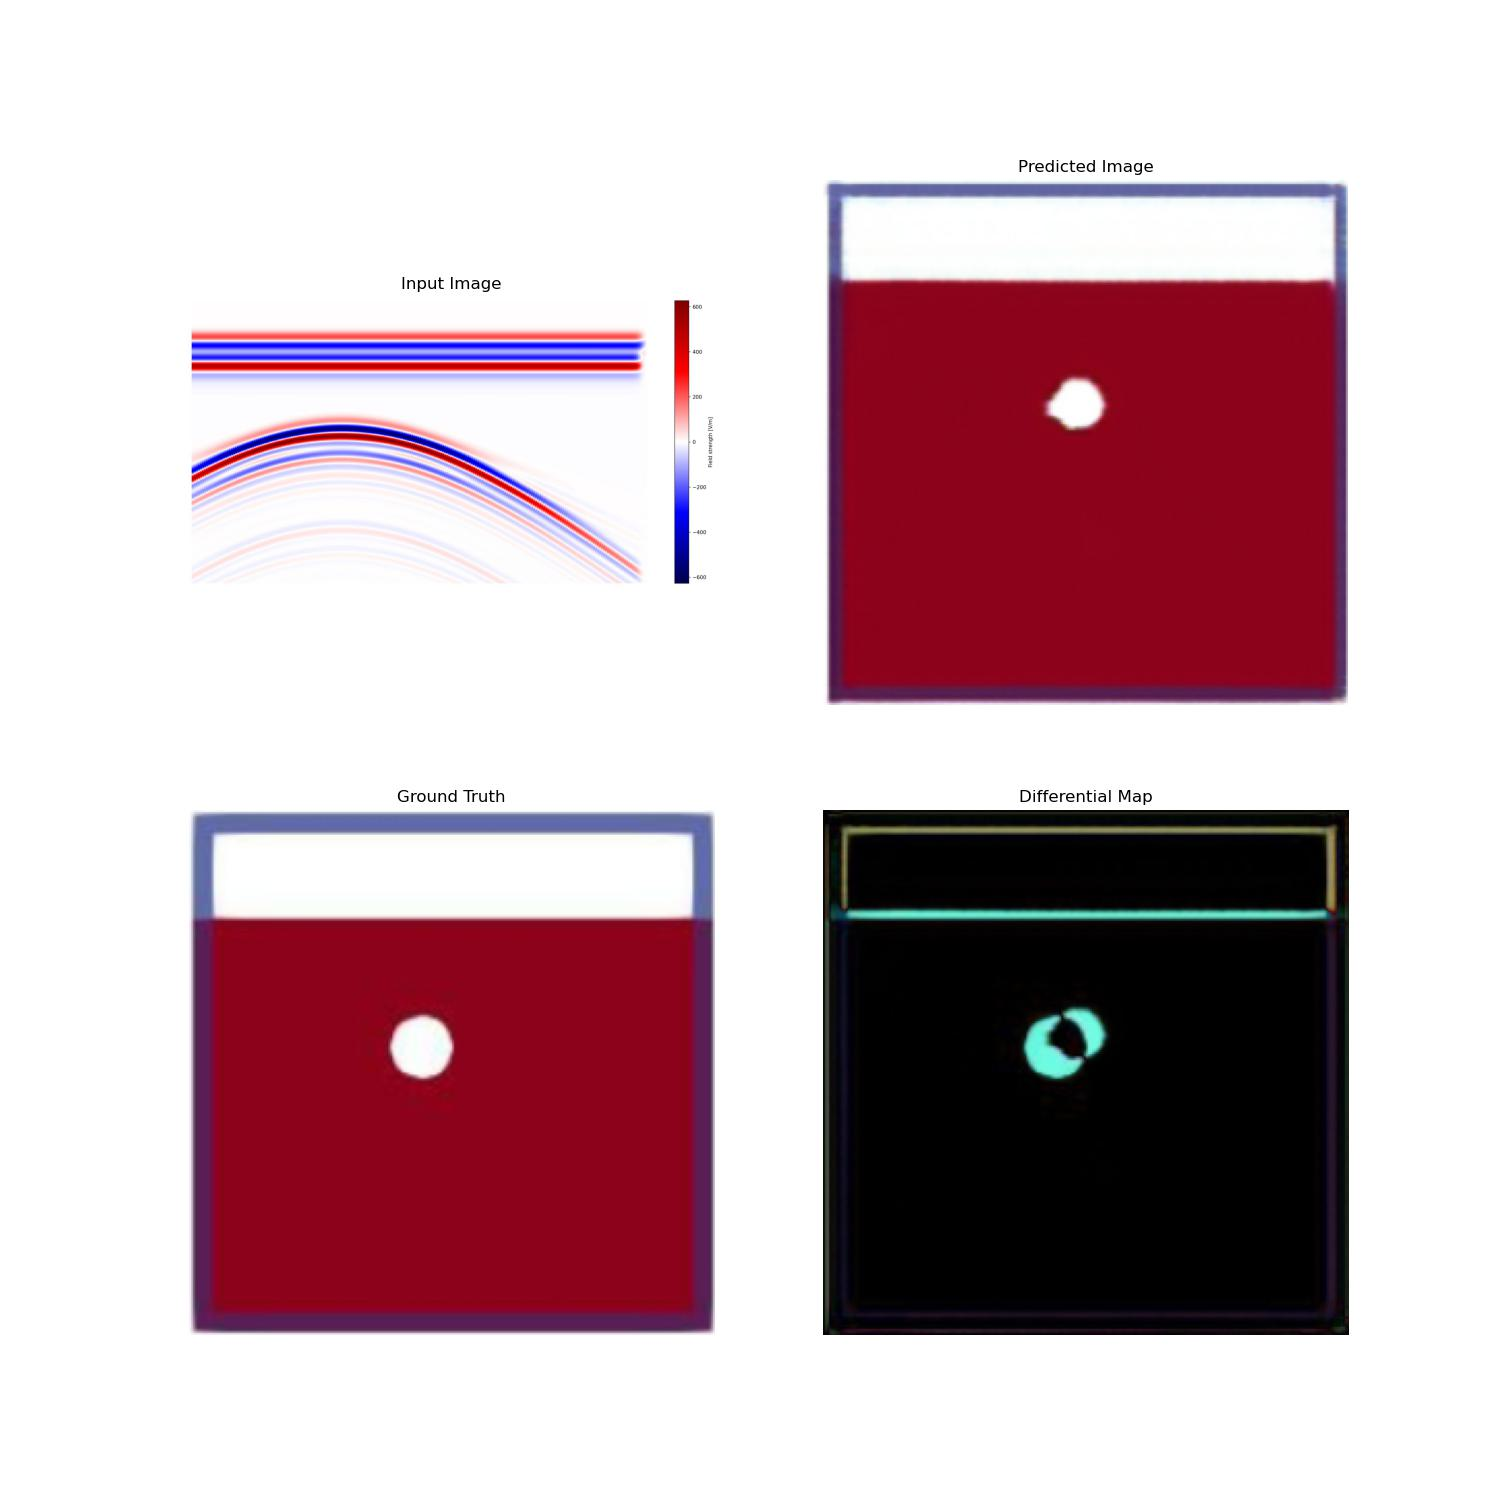
\includegraphics[scale=0.15]{gambar/diffMapLingkaran.jpg}
  \caption{Evaluasi Visual Data Variasi Bentuk Regular Lingkaran}
  \label{fig:diffmaplingkaran}
\end{figure}

Untuk variasi data dengan bentuk lingkaran akan diambil data kelima karena memiliki nilai evaluasi matriks yang lebih mendekati rata-rata variasi bentuk regular objek dari data lain. 
Evaluasi visual dari data dapat dilihat dari gambar \ref{fig:diffmaplingkaran}. 
Pada gambar evaluasi visual dapat dilihat bahwa irisan dari objek sintesis dengan objek asli cukup sedikit sehingga memiliki area error yang cukup luas. 
Hal ini menunjukkan bahwa output model hampir bisa menunjukkan posisi objek, namun masih belum bisa menunjukkan bentuk dan ukuran objek.

\begin{figure}[ht]
  \centering
  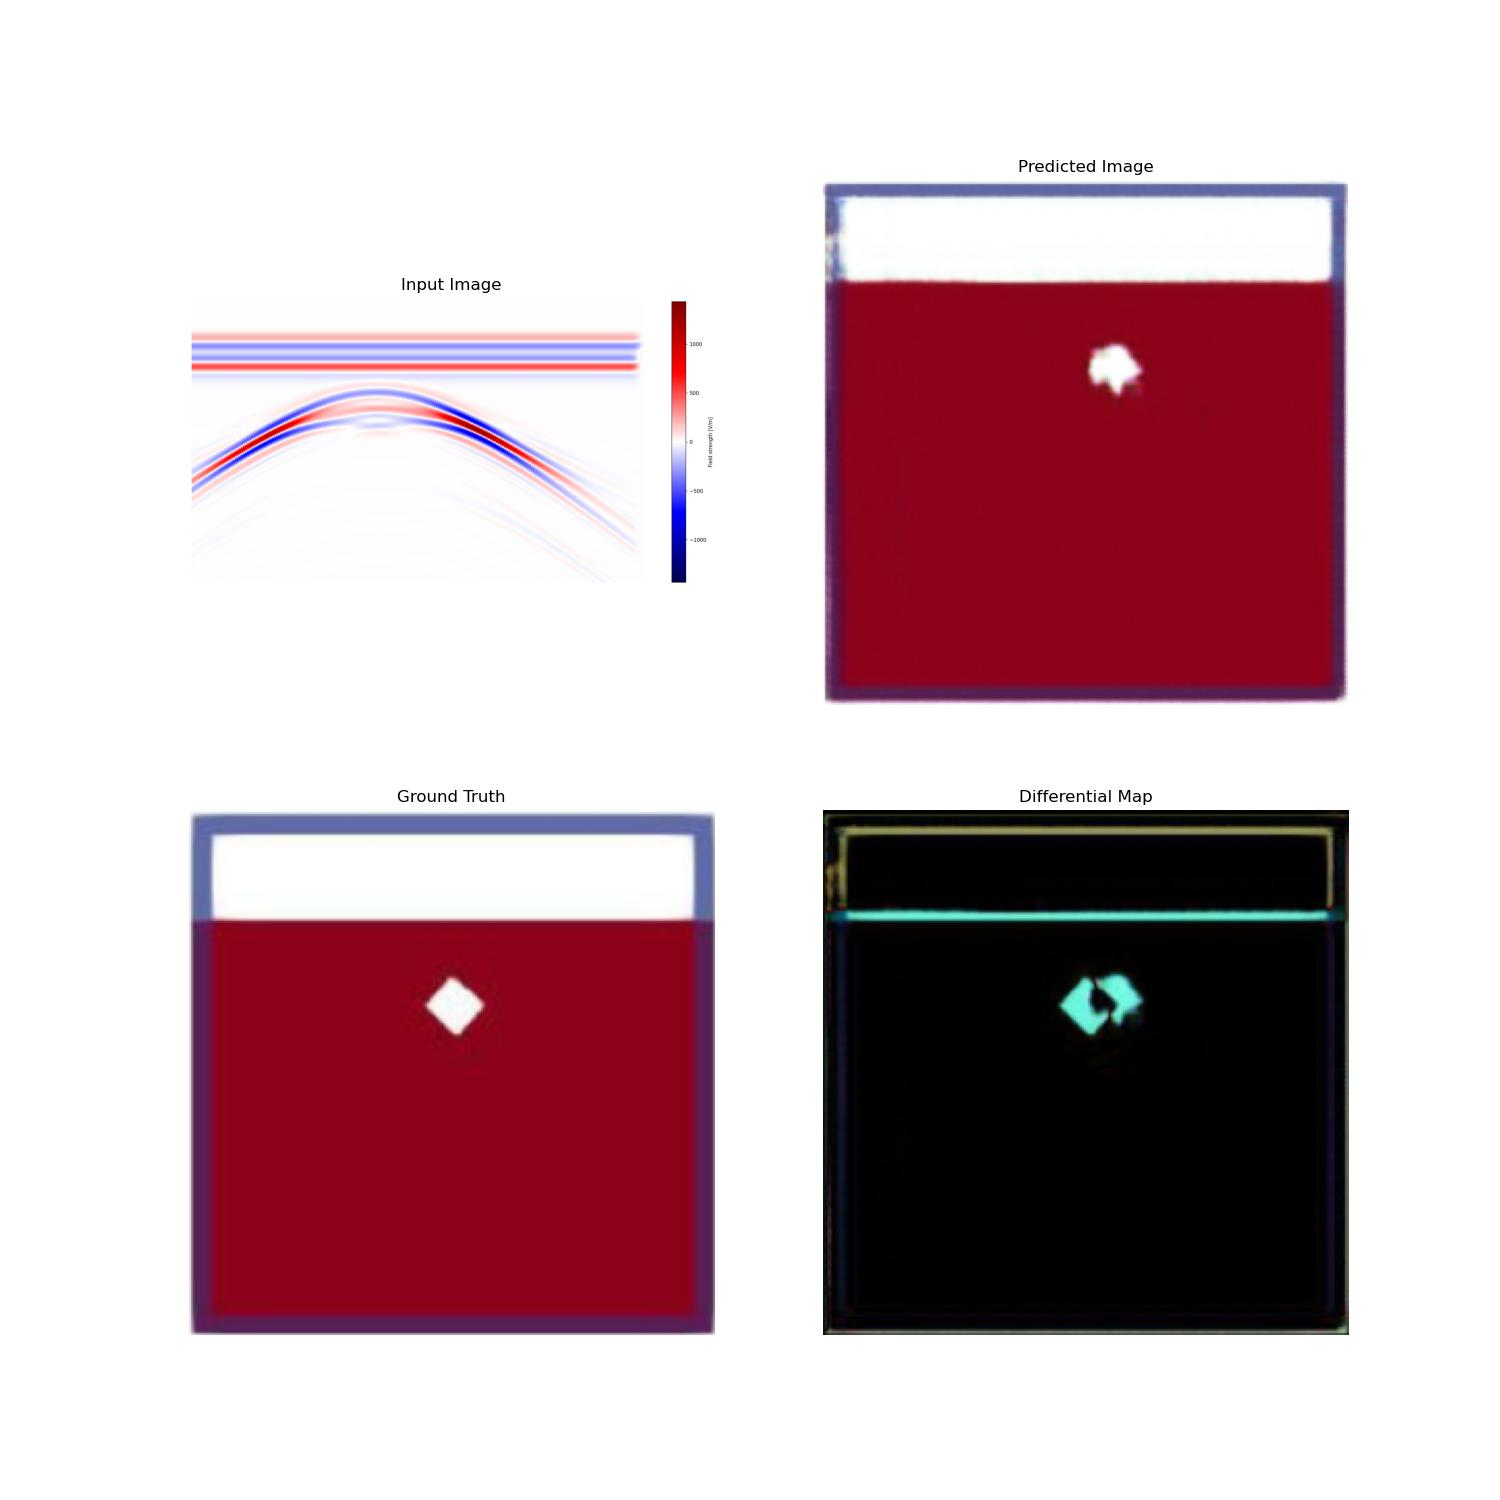
\includegraphics[scale=0.15]{gambar/diffMapSegi4.jpg}
  \caption{Evaluasi Visual Data Variasi Bentuk Regular Segi Empat}
  \label{fig:diffmapsegi4}
\end{figure}

Untuk variasi data dengan bentuk segi empat akan diambil data pertama karena memiliki nilai evaluasi matriks yang lebih mendekati rata-rata variasi bentuk regular objek dari data lain. 
Evaluasi visual dari data dapat dilihat dari gambar \ref{fig:diffmapsegi4}. 
Pada gambar evaluasi visual dapat dilihat bahwa irisan dari objek sintesis dengan objek asli cukup sedikit sehingga memiliki area error yang cukup luas. 
Hal ini menunjukkan bahwa output model hampir bisa menunjukkan posisi objek, namun masih belum bisa menunjukkan bentuk dan ukuran objek.
